\scanpage{3}

\diagram{\begin{array}{ll} A&\text{V.A.}\\ B&\text{duale}\end{array}}
\[
H^*(A)=\uuline{H}^{*}(A,\uuline{\Omega}^{*}_{A})
\qquad \text{\unsure{Ch.|Coh.} de Hodge-DeRham}
\]
\[
t_B=H^1(A,\uline{O}_A)
\]
\[
t_A=H^0(A,\Omega_A^1)^\vee\simeq H^{\unsure{n}}(A,\Omega_A^{n-1})
\]

\margin{$\unsure{S}_A$}
\diagram{\begin{tikzcd}[ampersand replacement=\&]
0\arrow[r,no head]\&t_A^\vee\arrow[r]\&\unsure{H^1}(A)\arrow[r]\&t_B\arrow[r]\&0
\end{tikzcd}}
\margin{extension canonique (du moins en \unsure{car.} $0$ !)}

Autre \unsure{interprétation} : Considérons l'extension \uline{universelle} de $A$ par un groupe vectoriel \inserted{$V$}, \deleted{elle} \unsure{se} \deleted{\unsure{définie}}\inserted{\unsure{classifie}} \inserted{une telle extension \unsure{se|est}} par
\[
H^1(A,\unsure{\uline{V}_A})=\deleted{\unsure{V}}\inserted{\operatorname{Hom}(H^1(A,\uline{O}_A)^\vee\unsure{,|\to}V)},
\]
\unsure{donc} l'extension universelle est
\diagram{\begin{tikzcd}[ampersand replacement=\&]
0\arrow[r,no head]\&\unsure{\mathbf{V}|W}(t_B^\vee)\arrow[r]\&E\arrow[r,no head]\&A\arrow[r,no head]\&0
\end{tikzcd}}
et passant aux espaces tangents on trouve une extension
\diagram{\begin{tikzcd}[ampersand replacement=\&]
0\arrow[r]\&t_B^\vee\arrow[r]\&t_E\arrow[r]\&t_A\arrow[r]\&0
\end{tikzcd}}
Je dis que cette extension n'est autre que $S_B$, (ce qui donne en passant
\[
t_E=H^1(B)
\]
)
et que de plus elle est \uline{\unsure{transposée}} de $S_A$, ce qui donne en passant
\[
\boxed{H^1(A)\text{ et }H^1(B)\text{ sont duaux l'un de l'autre}}
\]

\margin{\figure{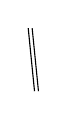
\begin{tikzpicture}\draw (0,0)--(-.08,.8);\draw (.05,0)--(-.03,.8);\end{tikzpicture}}}
\unsure{Plus préc.|Plus gén.}, il faut prouver que $H^*(A)$ et $H^*(B)$

\mspage{2}
